\subsection{Scale Analysis}
\label{sec:scale_analysis}

We examine the relationship between model scale and GPS reasoning performance using six models with known parameter counts: Qwen3-8B (8B), Qwen3-14B (14B), Mistral-Small-24B (24B), Qwen3-30B (30B total, 3B active), Mistral-Large (123B), and Qwen3-235B (235B total, 22B active).

\begin{figure}[htbp]
\centering
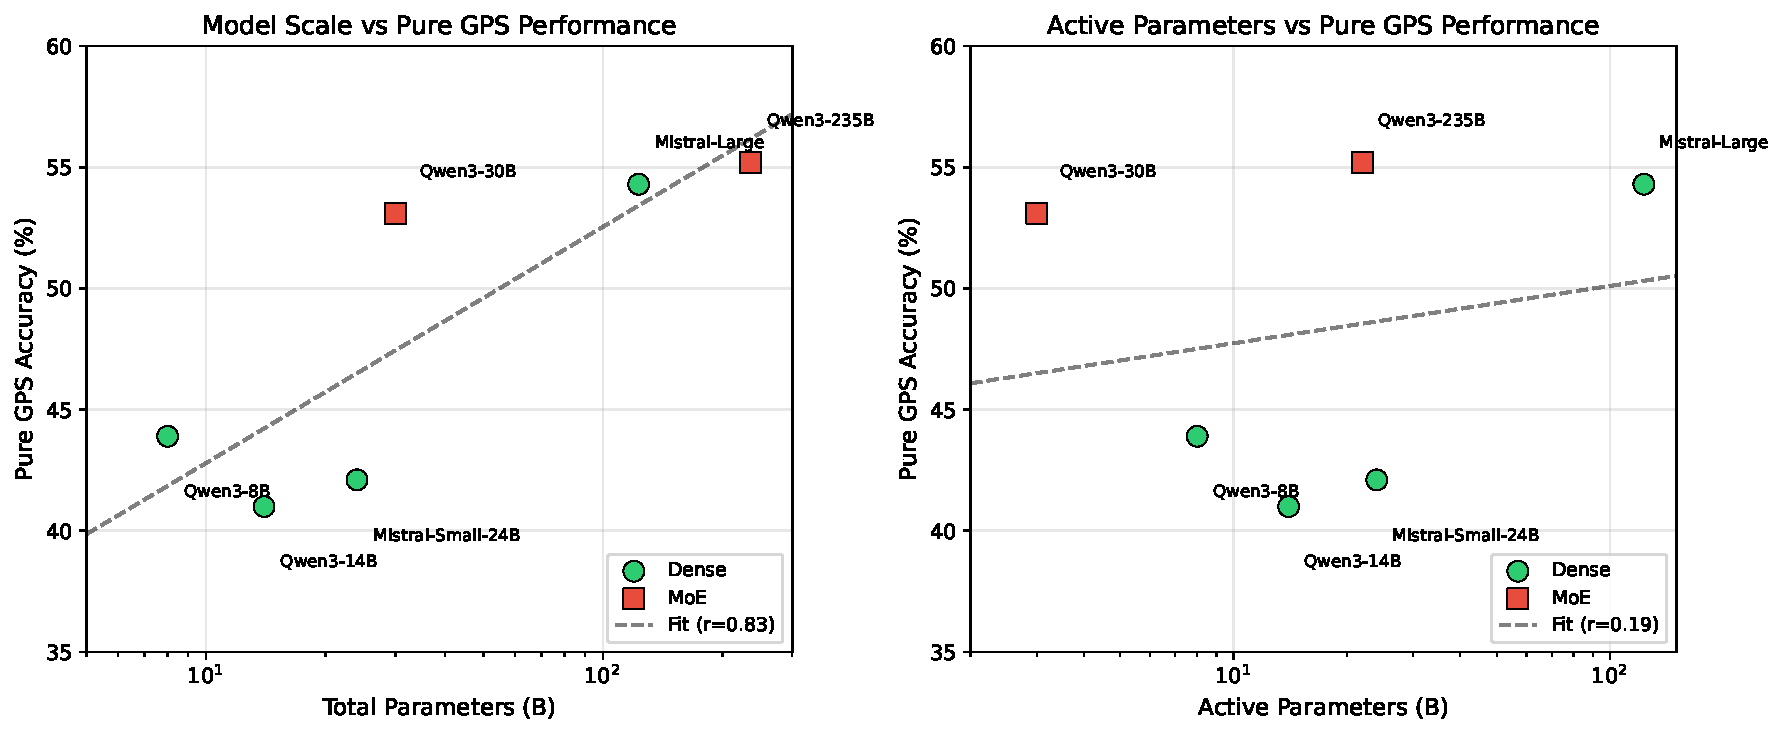
\includegraphics[width=\columnwidth]{figures/scale_analysis.pdf}
\caption{Model scale vs.\ Pure GPS accuracy. Left: total parameters show strong correlation (r=0.83). Right: active parameters show weak correlation (r=0.19), with MoE models (squares) achieving competitive accuracy using fewer active parameters.}
\label{fig:scale_analysis}
\end{figure}

\paragraph{Total vs.\ Active Parameters.}
Figure~\ref{fig:scale_analysis} reveals distinct scaling patterns for different metrics:
\begin{itemize}[leftmargin=*, itemsep=2pt]
    \item \textbf{Total parameters}: Strong correlation with Pure GPS accuracy (r=0.83, p=0.041), suggesting overall model capacity benefits coordinate computation.
    \item \textbf{Active parameters}: Weak correlation with Pure GPS accuracy (r=0.19, p=0.71), but strong correlation with Applied accuracy (r=0.84, p=0.034), indicating inference-time computation matters more for world knowledge tasks.
\end{itemize}

\begin{table}[htbp]
\centering
\caption{Scale analysis: model parameters vs.\ performance. MoE models are marked with active parameter counts in parentheses.}
\label{tab:scale_analysis}
\small
\begin{tabular}{lcccc}
\toprule
\textbf{Model} & \textbf{Params} & \textbf{Applied} & \textbf{Pure GPS} & \textbf{Type} \\
\midrule
Qwen3-8B & 8B & 62.2 & 43.9 & Dense \\
Qwen3-14B & 14B & 59.5 & 41.0 & Dense \\
Mistral-Small-24B & 24B & 59.8 & 42.1 & Dense \\
Qwen3-30B & 30B (3B) & 53.9 & 53.1 & MoE \\
Mistral-Large & 123B & 72.5 & 54.3 & Dense \\
Qwen3-235B & 235B (22B) & 69.8 & 55.2 & MoE \\
\bottomrule
\end{tabular}
\end{table}

\paragraph{MoE Efficiency.}
Mixture-of-Experts (MoE) models demonstrate remarkable efficiency for Pure GPS tasks. Qwen3-30B, despite activating only 3B parameters at inference (38\% of Qwen3-8B's dense parameters), achieves 53.1\% Pure GPS accuracy---9.2\% higher than Qwen3-8B (43.9\%). This suggests that total model capacity (for storing learned coordinate patterns) matters more than active computation for GPS reasoning.

However, MoE models show the opposite pattern on Applied tasks: Qwen3-30B (3B active) scores 53.9\% Applied accuracy, 8.3\% lower than Qwen3-8B (62.2\%). Applied reasoning appears to require more inference-time computation for integrating world knowledge with spatial queries.

\paragraph{Key Insights.}
\begin{enumerate}[leftmargin=*, itemsep=2pt]
    \item \textbf{Scaling helps computation}: Total parameter count correlates with Pure GPS accuracy (r=0.83), but diminishing returns appear above 100B parameters.

    \item \textbf{MoE architectures favor GPS}: MoE models achieve competitive Pure GPS scores while using significantly fewer active parameters, but underperform on Applied tasks requiring broader knowledge integration.

    \item \textbf{Dense models favor Applied}: Smaller dense models (8B-24B) show larger Applied-Pure GPS gaps (+17--18\%), indicating their capacity is better suited for world knowledge than coordinate computation.
\end{enumerate}
